\section{Introduction of the problem}
    \begin{frame}
    \frametitle{Physics of what we calculate}

    \begin{columns}
        \column{0.4\textwidth}
            \begin{wideitemize}
                \item Content of my Practical Training (Fachpraktikum)
                \item Hubbard Model Hamiltonian
                \item System under influence of external electric field
            \end{wideitemize}

        \column{0.5\textwidth}
            \makebox[\textwidth][c]{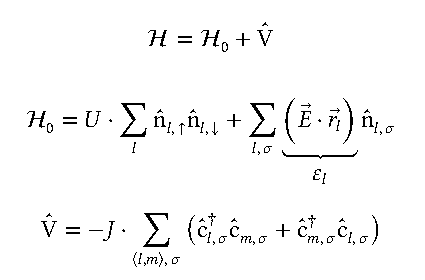
\includegraphics[width=\textwidth]{./main-content/physics/hamiltonian.pdf}}

    \end{columns}
\end{frame} 

\note[enumerate]{
    \item Hubbard-Model Hamiltonian with exterally applied electric field
    \item Hard-Core Bosinic Operators (will be explained in later slide, do not need to elaborate on)
    \item Spin-dependent lattice Model
    \item External electric field acts symmetric on both spin directions 
    \begin{itemize}
        \item This will be important later, multiple times
        \item All terms always need to be symmetric in terms of spin up/down
    \end{itemize}
}

\begin{frame}
    \frametitle{Physics of what we calculate}

    \begin{columns}
        \column{0.4\textwidth}
            \begin{wideitemize}
                \item 2-dimensional geometry
                \item Square lattice arrangement
                \item Computation for general size and field angle
            \end{wideitemize}
            
            \vspace{0.5cm}
            \begin{itemize}
                \item[Goal:]
                Approximate evaluation of time-evolution using Monte-Carlo Sampling
            \end{itemize}

        \column{0.5\textwidth}
            \makebox[\textwidth][c]{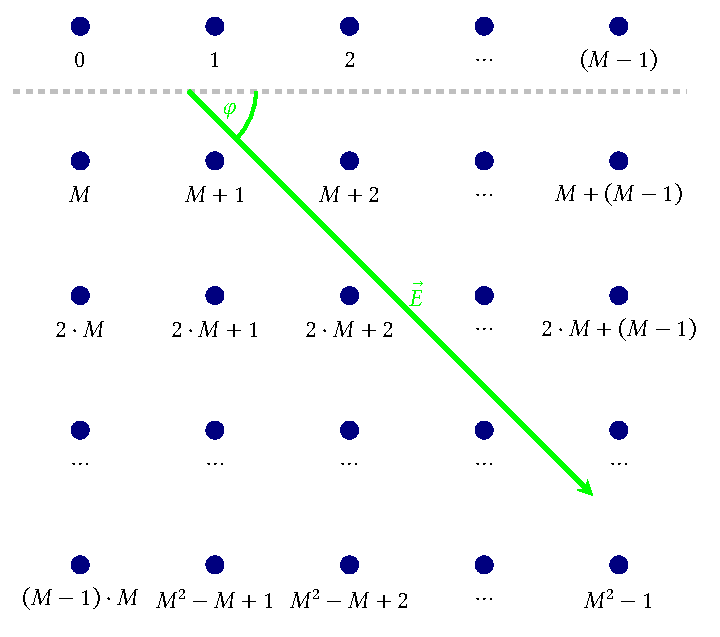
\includegraphics[width=.8\textwidth]{./main-content/physics/geometry.pdf}}
            
    \end{columns}
\end{frame}

\note[enumerate]{
    \item 2-dimensional square geometry
    \item Program supports already for general size inputs
    \item Thanks to the Monte-Carlo Sampling we can even efficiently evaluate larger systems already
}

\begin{frame}
    \frametitle{Physics of what we calculate}

    \begin{columns}
        \column{0.4\textwidth}
            \begin{wideitemize}
                \item Hard-Core Bosonic operators
                \begin{itemize}
                    \item (Would work analogously with Fermionic operators)
                \end{itemize}
                \item Two spin-degrees of freedom rewritten in alternate notation
            \end{wideitemize}

        \column{0.5\textwidth}
            \makebox[\textwidth][c]{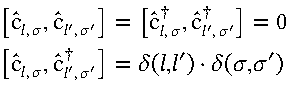
\includegraphics[page=1,width=.7\textwidth]{./main-content/physics/rewrite.pdf}}
            \makebox[\textwidth][c]{\includegraphics[page=2,width=.7\textwidth]{./main-content/physics/rewrite.pdf}}
            \makebox[\textwidth][c]{\includegraphics[page=3,width=.7\textwidth]{./main-content/physics/rewrite.pdf}}
            
    \end{columns}
\end{frame}

\note[enumerate]{
    \item Operators are hard-core bosonic
    \begin{itemize}
        \item standard commutation relations
        \item occupations are only either zero ore one
    \end{itemize}
    \item fermionic operators (anti-commutation) would work equivalent
    \item other notation to rewrite the two spin degrees of freedom into two operators of different dof makes it more readable and comfortable to apply computationally in some cases
}


    \begin{frame}[t]
    \frametitle{Working on paper: A Computer-Scientists view}

    Doing Theoretical Physics often requires lengthy analytical calculations
    \vspace{0.8em}

    \begin{columns}[t]
        \column{0.4\textwidth}
            \pause
            \textbf{Advantages} of working on paper:
            \begin{itemize}
                \item No barrier to entry (required Skill \& technology)
                \item Maximum liberty how to operate
                \item Fast iteration for high variation workload
                \item "Offline" available
            \end{itemize}
        
        \column{0.4\textwidth}
            \pause
            \textbf{Problems} of working on paper:
            \begin{itemize}
                \item Repetitive tasks not automizable
                \item Error-prone and time- consuming to fix mistakes
                \item Difficult \& non-standard to share/archive
                \item No version-control
                \item Need to produce final version anyway
            \end{itemize}
            
    \end{columns}

    % notes 
    \onslide % on all slides of frame
    \note[item] {
        Comparison of advantages/disatvantages of doing calculations "by hand"
    }
    \note[item] {
        Advantages
        \begin{itemize}
            \item No skills required to learn, writing is natural, every new symbol can just be written
            \item Operational Libery (cross out stuff as please, swap whatever without "proof")
            \item For completely different approaches no new tool is needed (lern that integral cannot be solved with a specific strategy that you tool doesn't support: out of luck)
            \item Hard to loose access to taken notes, produce them without internet/power
        \end{itemize}
    }
    \note[item] {
        Disatvantages
        \begin{itemize}
            \item Many tasks are repetetive, trivial and unfunny to do, paper cannot automize
            \item Sign errores, copy errors happen too often
            \item Sharing and archiving is non-standart. Many standarts exist for e.g. sharing latex
            \item No version-control (git): hard for people that are used to it like me. Cannot just do stuff and later revert if it didn't work
            \item Need to write the pretty version in the computer anyway
        \end{itemize}
    }
\end{frame}

\begin{frame}
    \frametitle{Examples from "Theoretical Solid State Physics"}

    \hspace{-1cm}
    \makebox[\textwidth][c]{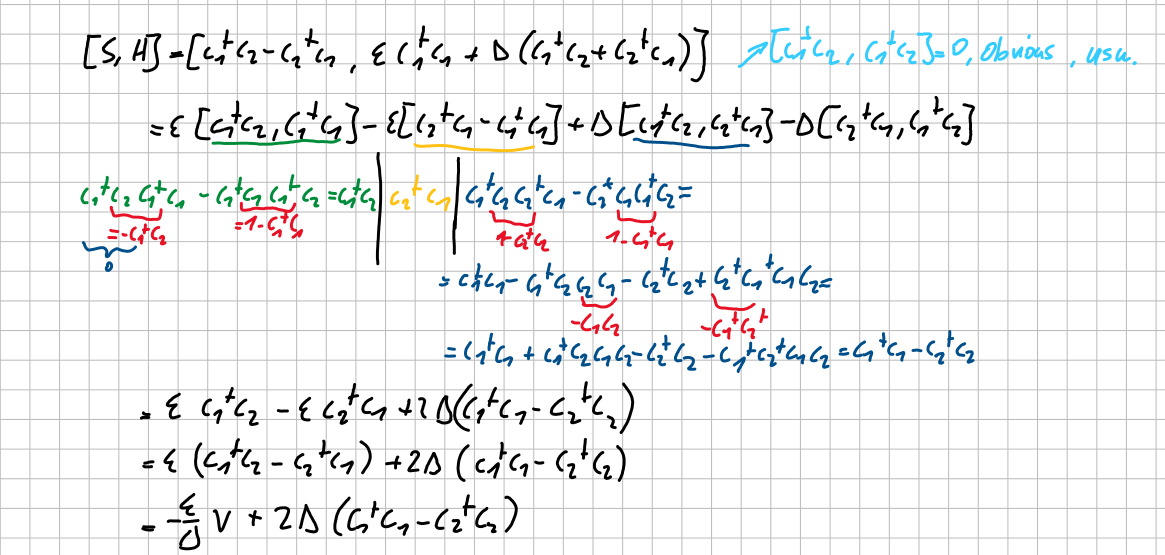
\includegraphics[width=0.85\textwidth]{math-manipulator-calculations/fkp_page_15.png}}
    
    % notes 
    \onslide % on all slides of frame
    \note[item] {
        From the lecture "Theoretical Solid State Physics" (Theoretische Festkörperphysik), helt by Markus Heyl in WS 22/23
    }
    \note[item] {
        Sheet 3, Problem 2: Schrieffer-Wolf transformation
    }
    \note[item] {
        Rather simple calculation, still contains sing mistakes (that here luckily averaged out)
    }
\end{frame}

\begin{frame}
    \frametitle{Examples from "Theoretical Solid State Physics"}

    \hspace{-1cm}
    \makebox[\textwidth][c]{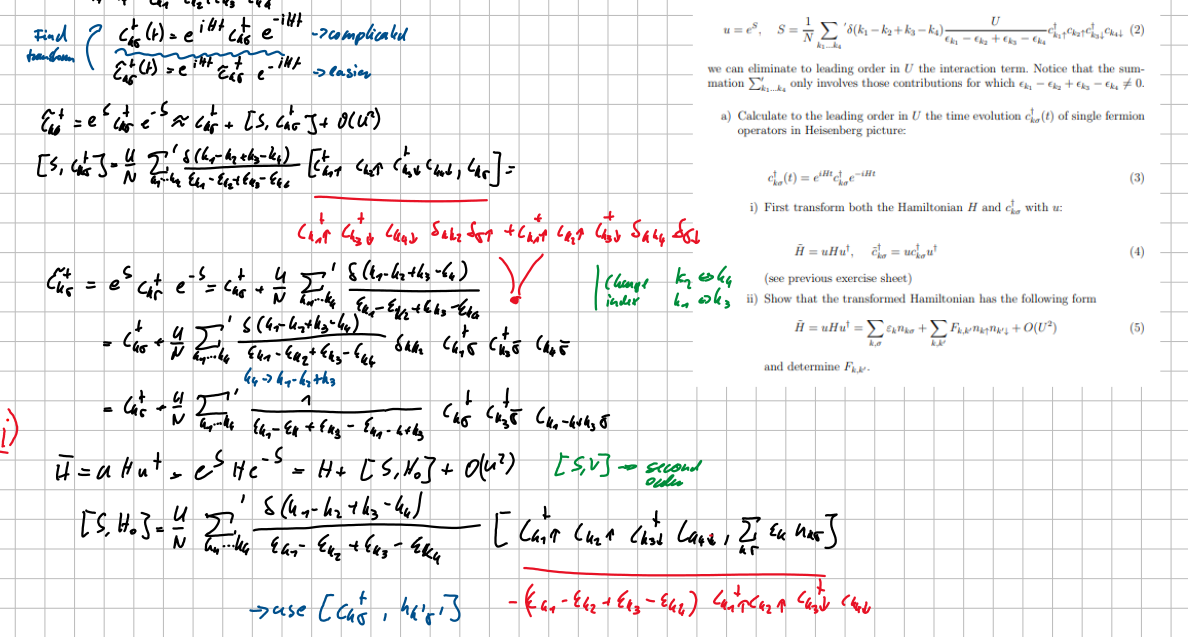
\includegraphics[width=0.85\textwidth]{math-manipulator-calculations/fkp_page_33.png}}
    
    % notes 
    \onslide % on all slides of frame
    \note[item] {
        From the lecture "Theoretical Solid State Physics" (Theoretische Festkörperphysik), helt by Markus Heyl in WS 22/23
    }
    \note[item] {
        Sheet 8, Problem 1: Schrieffer-Wolf transformation of the Hubbard Model
    }
    \note[item] {
        Just written down steps done by someone else (Tutor/other pupil, often shared the terms to calculate them all, still time)
    }
\end{frame}

\begin{frame}
    \frametitle{Examples from the Practical Training}

    \begin{columns}
        \column{0.4\textwidth}
            \begin{itemize}
                \item Goal: produce time evolution of operator
                \onslide<2->
                \item Uses calculation in Interaction Picture
                \onslide<3->
                \item Workflow:
                \begin{itemize}
                    \item Inserting Definitions
                    \item Expanding
                    \item Ordering
                    \item Rewriting efficiently
                \end{itemize}
            \end{itemize}

        \column{0.4\textwidth}
            \onslide<1->
            \makebox[\textwidth][c]{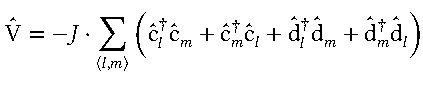
\includegraphics[page=1,width=.9\textwidth]{./main-content/paper/V_interaction_picture.pdf}}
            \vspace{0.3em}
            \onslide<2->
            \makebox[\textwidth][c]{\includegraphics[page=2,width=.9\textwidth]{./main-content/paper/V_interaction_picture.pdf}}
            
    \end{columns}

    % notes 
    \onslide % on all slides of frame
    \note[item] {
        Want to calculate the Time-Evolution of the operator V in the interaction Picture
    }
    \note[item] {
        Basically comes down to inserting definitions (however already derived from MM)
    }
    \note[item] {
        Distributing and re-ordering is a painful, time-intensive process
    }
\end{frame}


\section{Solutions: Off the shelf}
    \begin{frame}[t]
        \frametitle{Paper-like writing on digital devices}
        
        \vspace{-0.5em}
        \begin{itemize}
            \item Can give benefits that paper lacks
            \begin{itemize}
                \item Copy/Paste
                \item Collaborate
                \item Convert to text
                \item Searching and ordering large amounts of notes
            \end{itemize}
            \pause
            \item HOWEVER
            \begin{itemize}
                \item Still no proper automatization
                \item Easily access is lost when using proprietary technology
                \item "Vendor-Locking"
            \end{itemize}
        \end{itemize}
        \pause
        \begin{block}{TIP:}
            Always export to a standard format (like pdf) for manual backup!
        \end{block}


        % notes 
        \onslide % on all slides of frame
        \note[item] {
            Taking notes digially can have many benefits
        }
        \note[item] {
            OneNote, Xournalpp, Notion and many more examples
        }
        \note[item] {
            Still lacks "true" automatization
        }
        \note[item] {
            Great danger of Vendor-Locking, losing access
            \begin{itemize}
                \item Cloud-Driven offers do not work without internet
                \item Often times even tied to the device (Apple-Notes I-pad, personal experience with one-note)
                \item Countless stories about providers ending support, users getting blocked and more
            \end{itemize}
        }
        \note[item] {
            Conclusion: very great choice to boost productivity. But TIP: archive everything as pdf if you ever plan to use it later. It may save you weeks of work/complete loss of data.
        }
    \end{frame}

    \begin{frame}
        \frametitle{Computer-Algebra Systems}

        \begin{itemize}
            \onslide<1->
            \item Proprietary Software (Often payed):
            \onslide<2->
            \begin{itemize}
                \item Wolfram-Alpha
                \item Mathematica
                \item Chat-GPT
                \item ...
            \end{itemize}
            \onslide<1->
            \item Standalone Online Calculators
            \onslide<2->
            \begin{itemize}
                \item Integralrechner.de (Integral-Calculator)
                \item Matrix-Calculators
                \item ...
            \end{itemize}
            \onslide<3->
            \item ... and many more 
        \end{itemize}

        % notes 
        \onslide % on all slides of frame
        \note[item] {
            There exist already countless possible attempts at solving the worlds problems
        }
        \note[item] {
            All of them are great at what they are designed for, I will not attempt competing with any of the m in terms of any metric except maybe usability (and probably still fail)
        }
        \note[item] {
            Chat-GPT is included in the list, because it can do many calculations by now, however is extremely unreliable
        }
        \note[item] {
            Central, reoccuring Problems (multiple ore some for everything)
            \begin{itemize}
                \item Paid access
                \item Non-reliable
                \item Difficult to "cite"/ use in paper/thesis
                \item Limited in scope, because software is very spezialized to the task
                \item Require training/ prior (export) knowlede to properly take advantage of
            \end{itemize}
        }
    \end{frame}
